\chapter{Validazione del codice}
\label{ch:Validazione}

Per collaudare %mettere alla prova
il metodo risolutivo sono stati implementati vari potenziali di cui si conosce la soluzione analitica per poter confrontare i risultati numerici con l'evoluzione esatta. In tutte le simulazioni è stato utilizzato come operatore di evoluzione quello in eq. (\ref{eq:LT_2}), considerato come il miglior compromesso tra precisione e costo computazionale.


\section{Particella libera}
\label{sec:free}

\subsection{Pacchetto d'onde gaussiano}
\label{sec:WP_gaussiano}

Si ricorda la definizione di pacchetto d'onda per le onde piane, poiché è stato scelto come principale stato iniziale all'interno delle simulazioni.
\begin{equation}
    \centering
    \psi(q, 0) = \frac{1}{\sqrt{2 \pi}} \int_{- \infty}^{+ \infty} dk \; g(k) \exp \left(ikq\right) \, \text{,}
    \label{eq:WP}
\end{equation}
dove $g(k)$ rappresenta una distribuzione di probabilità che fissa i contributi per ogni valore di $k$.
Per un pacchetto gaussiano\footnote{Dove $g(k)$ prende la forma di distribuzione gaussiana} e sostituendo le definizioni
\begin{equation}
    \hbar k \equiv p - p_0 \, \text{,}   \quad q \equiv x - x_0 \, \text{,}
    \label{eq:def_kq}
\end{equation}
l'eq. (\ref{eq:WP}) si riduce a 
\begin{equation}
    \centering
    \psi(x, 0) = \left( \frac{2}{ \pi \sigma^2} \right)^{\nicefrac{1}{4}} \exp \left(-i \frac{p_{0}}{\hbar} (x -x_0)\right) \exp \left(-\frac{(x -x_0)^2}{\sigma^{2}}\right) \, \text{,}
    \label{eq:WP_gaus}
\end{equation}
dove $p_0$ rappresenta lo sfasamento del pacchetto nello spazio dei momenti ed è la grandezza che controlla l'energia cinetica associata al pacchetto $T = p_{0}^{2} / 2m$. In figura {\ref{fig:free_p_view}} viene riportato un esempio.

\begin{figure}
    \centering
    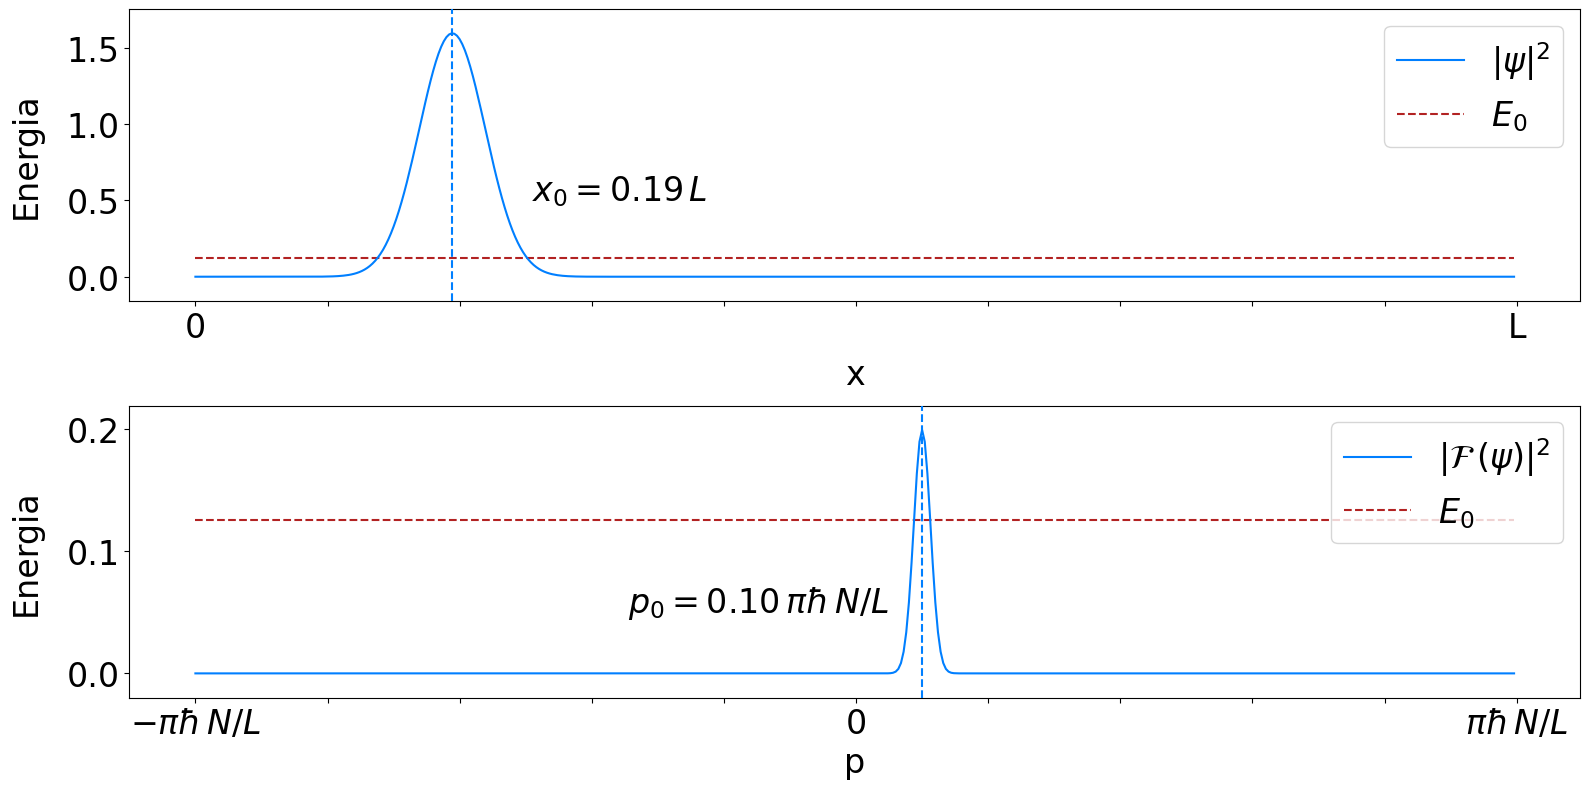
\includegraphics[width = \textwidth]{immagini/free_p_view.png}
    \caption{Rappresentazione dello stato inziale per un pacchetto gaussiano di onde piane, sia nello spazio diretto sia nello spazio dei momenti.}
    \label{fig:free_p_view}
\end{figure}

\subsection{Evoluzione analitica}

Con potenziale di particella libera si intente una configurazione a potenziale costante $V(x) = 0$. In tale configurazione si può considerare la soluzione analitica per l'evoluzione di un pacchetto d'onde del tipo in eq. (\ref{eq:WP_gaus}). 
Data l'eq. (\ref{eq:Sc_1D}), con $V(x) = 0$, questa è risolta per ogni funzione del tipo
\begin{equation}
    \centering
    \psi(x, t) = A \exp \left(i(kx - \omega t)\right) \qquad \text{con}  \quad \omega = \frac{\hbar k^2}{2m} \, \text{.}
    \label{eq:plane_wave}
\end{equation}
Dal principio di sovrapposizione si ottiene che
\begin{equation}
    \centering
    \psi(q,t) = \frac{1}{\sqrt{2 \pi}} \int_{- \infty}^{+ \infty} dk \; g(k) \exp \left(i(kq - \omega t)\right) \, \text{.}
    \label{eq:WP_ev}
\end{equation}
Considerando un pacchetto gaussiano e sostituendo le definizioni in eq. (\ref{eq:def_kq}), si ottiene una funzione analitica per l'evoluzione del pacchetto nel tempo \cite{CT:QM}
\begin{equation}
    \centering
    \psi(x,t) = 
    \left( \frac{2 \sigma^2}{\pi} \right)^{\nicefrac{1}{4}} 
    \left( \sigma^4 + \frac{4 \hbar^2 t^2}{m^2}   \right)^{\nicefrac{-1}{4}}
    \exp \left(i \frac{p_0}{\hbar} x\right) 
    \exp \left( - \frac{\left[ x - p_0 t / m \right]^{2}} {\sigma^2 - 2 i \hbar t / m} \right)
    e^{i \phi} \, \text{,}
    \label{eq:WP_gaus_ev}
\end{equation}
\begin{equation}
    \centering
    \text{con} \quad \phi = - \frac{1}{2} \arctan (\frac{2 \hbar t}{m \sigma_0^2}) - \frac{p_0^2}{2 m \hbar} t  \, \text{.}
\end{equation}
In figura (\ref{fig:free_ev}) si riporta il confronto tra la soluzione numerica e quella analitica per alcuni tempi successivi.

\begin{figure}
    \centering
    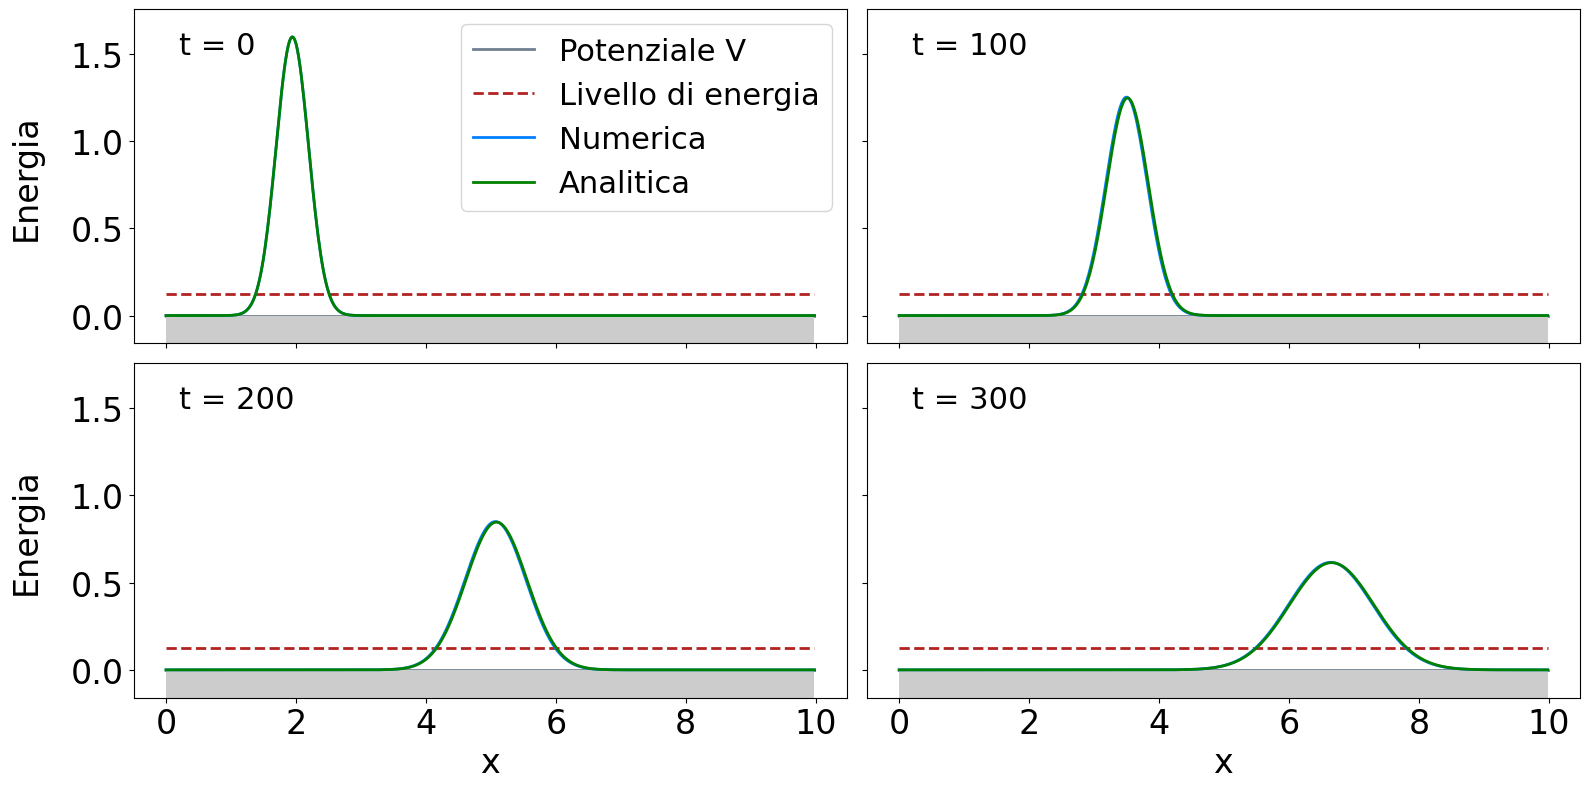
\includegraphics[width = \textwidth]{immagini/free_ev.png}
    \caption{Confronto tra soluzione numerica e soluzione analitca per una particella libera. Si può notare un'ottima sovrappsozione tra le due.}
    \label{fig:free_ev}
\end{figure}


\section{Oscillatore armonico}
\label{sec:arm}

L'oscillatore armonico quantistico è definito da 
\begin{equation}
    \centering
    V(x) = \frac{1}{2} m \omega^2 (x -x_0)^2 \, \text{.}
\end{equation}
Si ricordano i principali risultati ottenuti dalla soluzione dell'equazione di Schr\"odinger stazionaria
\begin{equation}
    \centering
    E_n = (\frac{1}{2} + n) \hbar \omega \, \text{,} \qquad \psi_{n} = \left( \frac{\beta^2}{\pi} \right)^{\nicefrac{1}{4}} \frac{1}{\sqrt{2^{n} \, n!}} \exp \left(-\frac{- \beta^2 x^2}{2}\right) H_{n}(\beta x) \, \text{,}
    \label{eq:arm_res}
\end{equation}
\begin{equation}
    \centering
    \text{con}  \quad \beta = \sqrt{\frac{m \omega}{\hbar}} \, \text{.}
\end{equation}
È noto che se si considera l'eq. (\ref{eq:U}) per gli stati stazionari questa si riduce a 
\begin{equation}
    \centering
    \psi_{n}(x, t) = \exp \left( - \frac{i}{\hbar} E_n t \right) \psi_{n} (x,0)      \, \text{.}
    \label{eq:ev_eigenstate}
\end{equation}
Se inoltre si considera come stato iniziale una combinazione lineare di autostati è possibile trovare l'evoluto temporale combinando le evoluzioni di ogni singolo autostato
\begin{equation}
    \centering
    \psi(x, t) = \sum_{k} c_{k} \, \exp \left( - \frac{i}{\hbar} E_k t \right) \psi_k (x,0) \qquad \text{con} \quad\psi(x,0) = \sum_{k} c_{k} \,  \psi_k (x,0)        \, \text{,}
    \label{eq:ev_combinazione}
\end{equation}
che è una funzione analitica esatta.

\textcolor{red}{ In figura %(\ref{fig:superpos}) 
riportano il confronto tra la soluzione numerica e l'evoluzione analtica per la sovrappoizione di auotostati dell'oscillatore armonico
\begin{equation}
    \centering
    \psi(x, 0) = \frac{1}{\sqrt{2}} \left( \ket{0} + \ket{1} \right)   \, \text{.}
    \label{eq:superpos}
\end{equation} 
}

\section{Stati coerenti}
\label{sec:coherent}

Con stati coerenti \cite{CT:QM} si intendono gli autostati dell'operatore di distruzione dell'oscillatore armonico. Sono divenuti celebri, poiché vennero utilizzati da Schr\"odinger come dimostrazione del principio di corrispondenza. Tali stati, infatti, sono caratterizzati da una dinamica molto simile al comportamento oscillatorio di un oscillatore armonico classico. 

Non esiste una definizione analitica per gli stati coerenti, poiché sono definiti tramite una sovrapposizione infinita, del tipo in eq. (\ref{eq:ev_combinazione}), di autostati di oscillatore armonico nel seguente modo
\begin{equation}
    \centering
    \ket{\alpha} = \exp \left(- \frac{|\alpha|^2}{2}\right) \sum_{n=0}^{+ \infty} \left( \frac{\alpha^n}{n!} \right) \ket{n} \, \text{.}
    \label{eq:def_coherent}
\end{equation} 
Numericamente non è possibile estendere la somma a $+\infty$, per questo è necessario troncarla ad un valore finito, all'interno del codice è stato fissato a 170.

L'evoluzione analitica per il modulo quadro di uno stato coerente corrisponde ad una traslazione rigida di una gaussiana con 
\begin{equation}
    \centering
    \expval{x}_{t} = A \, cos(\theta - \omega t) \, \text{,} \quad
    \expval{p}_{t} = m \omega A \, sen(\theta - \omega t) \qquad
    \text{dove} \quad A = \sqrt{\frac{2 \hbar}{m \omega}} |\alpha| \, \text{,}
    \label{eq:coherent_an}
\end{equation}
che corrispondono alle soluzioni classiche dell'oscillatore armonico.

In figura (\ref{fig:coherent_ev}) è riportato il confronto tra la soluzione analitica e numerica per l'evoluzione di uno stato coerente, mentre in sezione (\ref{sec:Wp_arm}) si studia l'evoluzione di pacchetto gaussiano di onde piane anche in confronto ad uno stato coerente.

\begin{figure}
    \centering
    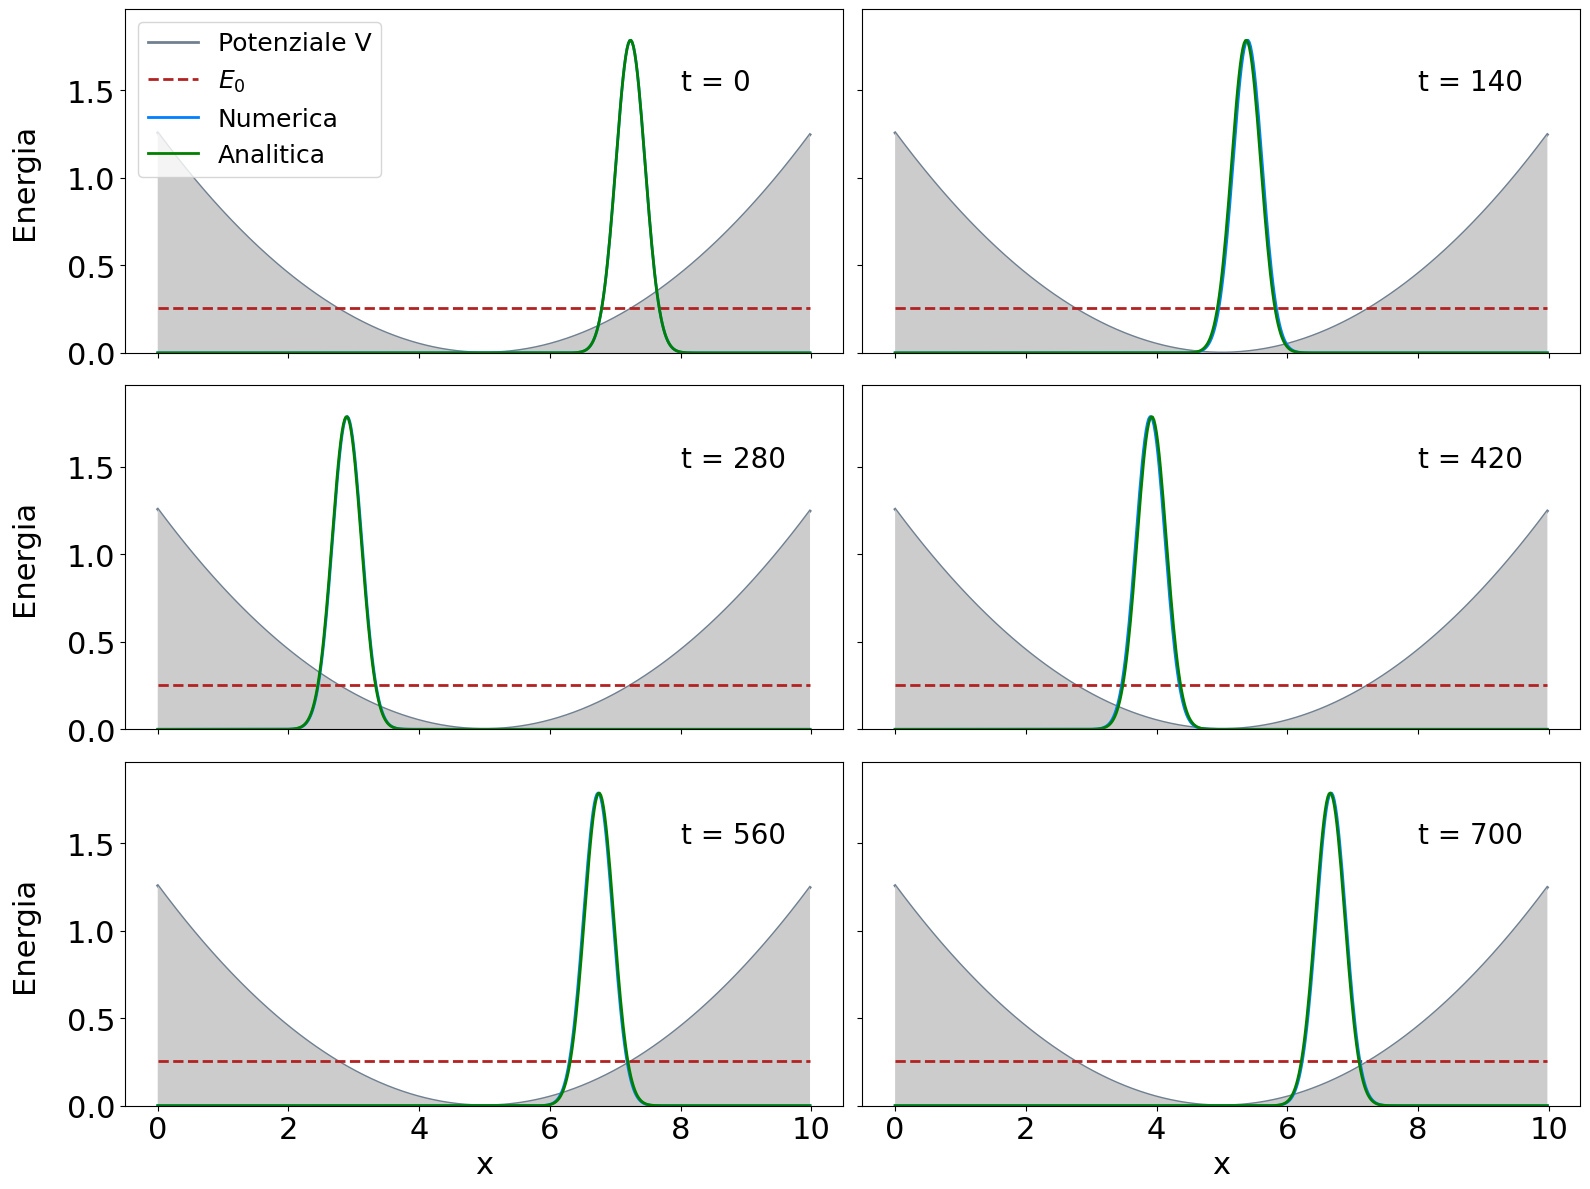
\includegraphics[width = \textwidth]{immagini/coherent_ev.png}
    \caption{Confronto tra soluzione numerica e soluzione analitica per uno stato coerente. Si noti come le dimensioni del pacchetto di forma gaussiana non vengano deformate durante l'evoluzione.}
    \label{fig:coherent_ev}
\end{figure}



\section{Potenziale di P\"oschl-Teller}
\label{sec:RL}

Il potenziale di P\"oschl-Teller (PT), applicato nel contesto della meccanica quantistica, prende la forma 
\begin{equation}
    \centering
    V(x) = -\frac{\hbar^2 \alpha^2}{2m} \frac{\nu (\nu + 1)}{\cosh^2 \alpha x} \quad \text{.}
    \label{eq:pot_PT}
\end{equation}
Questo potenziale è di particolare importanza poiché si può dimostare che $\forall \nu$ il coefficiente di trasmissione, $T$, per una funzione d'onda incidente sul potenziale risulta essere pari a $1$. Per questo gli viene attribuito l'aggettivo \textsl{reflectionless}.   
Come per il potenziale armonico è possibile risolvere l'equazione agli autovalori per PT con un metodo algebrico, definendo gli operatori di innalzamento e abbassamento, quindi risolvere analiticamente il problema per una qualsiasi combinazione di autostati in analogia con quanto fatto in precedenza. \cite{Jaffe:RL_sol}

Fissando  $\nu = 1$ si ottengono gli autostati e autovalori
\begin{equation}
    \centering
    \psi_{k}(x) = \left[ \frac{i k - \alpha \tanh (\alpha x)}{ik + a}\right] \exp(ikx)  \; \text{,} \quad E_k = \frac{\hbar^2 k^2}{2 m } \quad \text{con} \; k \in \mathbb{R} \, \text{,}
\end{equation}
che generano uno spettro continuo e infinito. Si può, dunque, costruire un pacchetto d'onde di autostati 
\begin{equation}
    \centering
    \psi(x, t) = \frac{1}{\sqrt{2 \pi}} \int_{-\infty}^{+\infty} dk \, A(k) \, \psi_{k}(x) \exp \left(- \frac{i}{\hbar} E_k t \right) \, \text{,}
    \label{eq:WP_RL_def}
\end{equation}
si ricorda che $p - p_0 \equiv \hbar k$.
Fissando $A(k) = (ik + \alpha) \phi_0(k)$, dove $\phi_0(k)$ è la trasformata di Fourier dell'eq. (\ref{eq:WP_gaus}) e risolvendo l'integrale si ottiene la soluzione per l'evoluzione di un pacchetto d'onde gaussiano di autostati di PT
\begin{equation}
    \centering
    \psi(x, t) = N \left[i \frac{p_0}{\hbar} - \frac{x - x_0 - v_{g}t}{ \sigma_0 s_t} - \alpha \tanh (\alpha x) \right] \psi_{G}(x,t)    \, \text{,}
    \label{eq:WP_RL_ev}
\end{equation}
\begin{equation}
\text{con} \quad s_t = \frac{\sigma_0}{2} \left(1 + i \frac{2 \hbar t}{ m \sigma_0^2} \right)
\end{equation}
e dove $\psi_{G}(x,t)$ si riferisce all'evoluzione libera di un pacchetto gaussiano di onde piane, $v_g = p_0 / m$ è la velocità di gruppo.\cite{Mousavi:PL_WP}

In figura (\ref{fig:WP_RL}) si riporta il confronto tra la soluzione numerica e la soluzione analitica, riscontrando una quasi perfertta sovrapposizione.

\begin{figure}
    \centering
    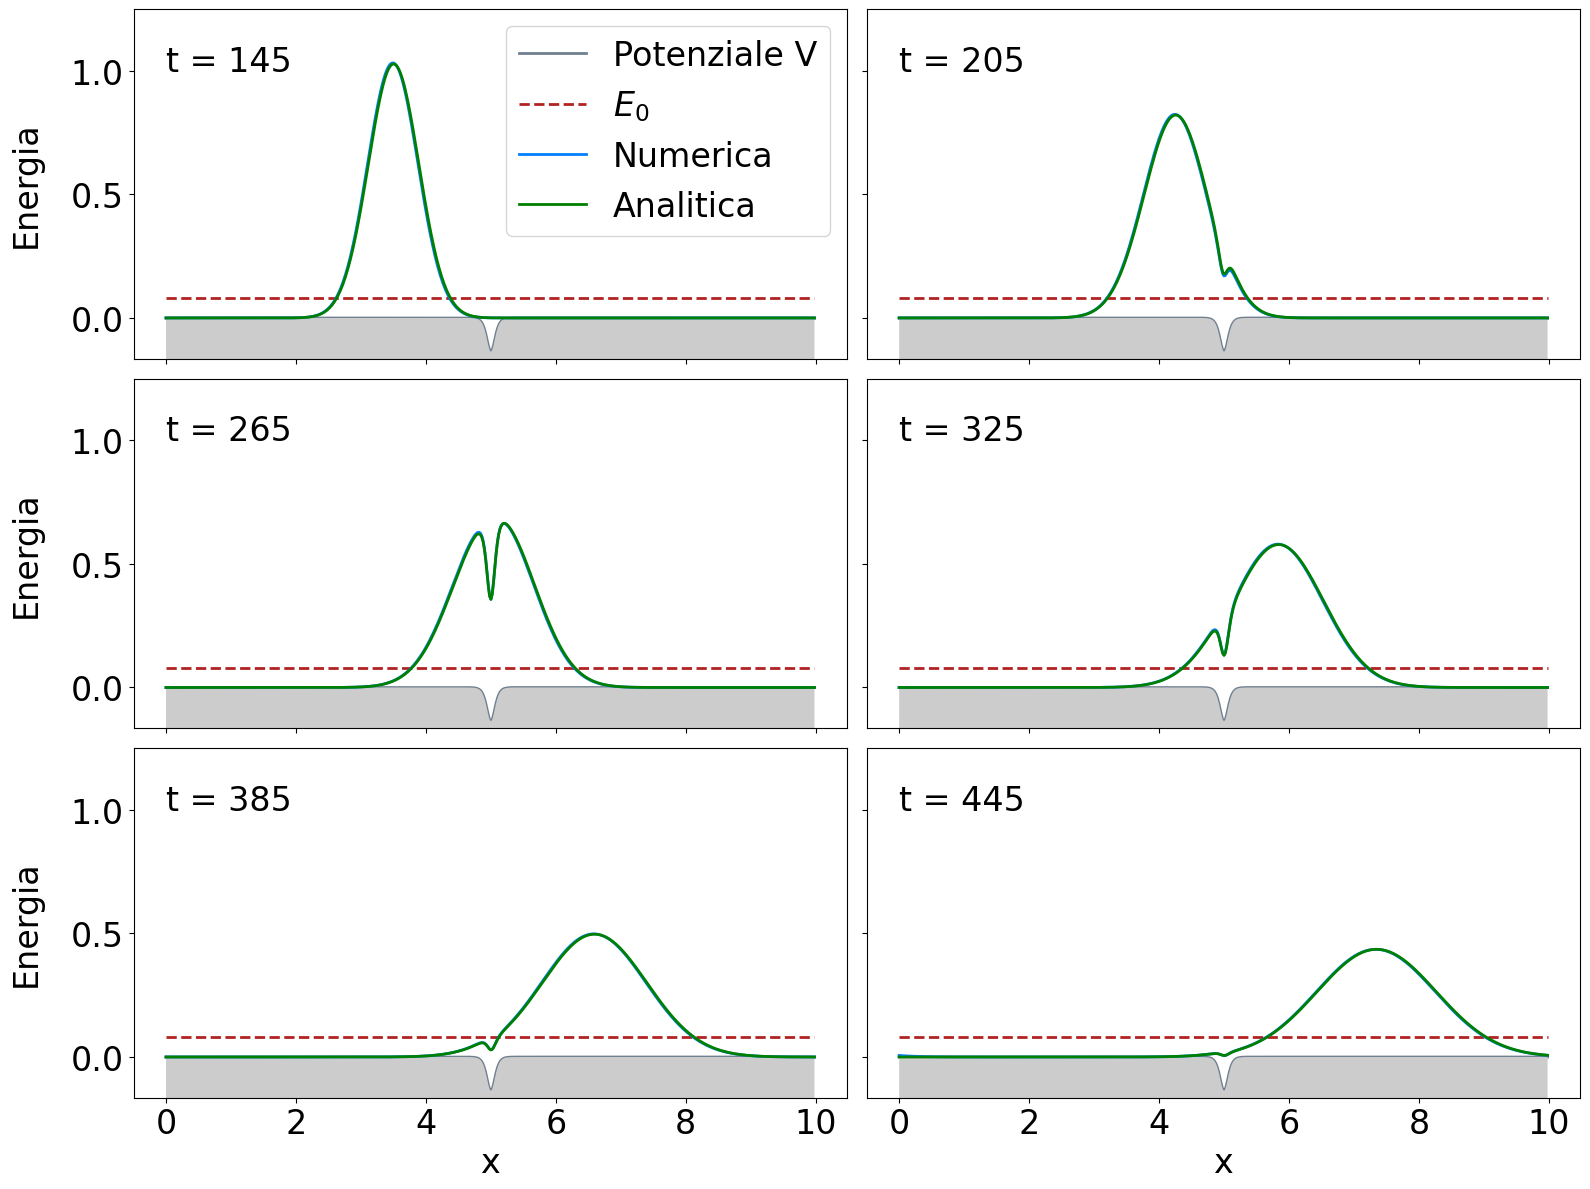
\includegraphics[width = \textwidth]{immagini/WP_RL.png}
    \caption{Confronto tra soluzione numerica e soluzione analitica per un pacchetto gaussiano di autostati di PL. Ancora una volta si ottiene un ottimo accordo tra la simulazione numerica e l'evoluzione esatta.}
    \label{fig:WP_RL}
\end{figure}

